\begin{figure*}[ht!]
\begin{center}% note that \centering uses less vspace...
\resizebox{2\columnwidth}{!}{%
\begin{tabular}{lllll}


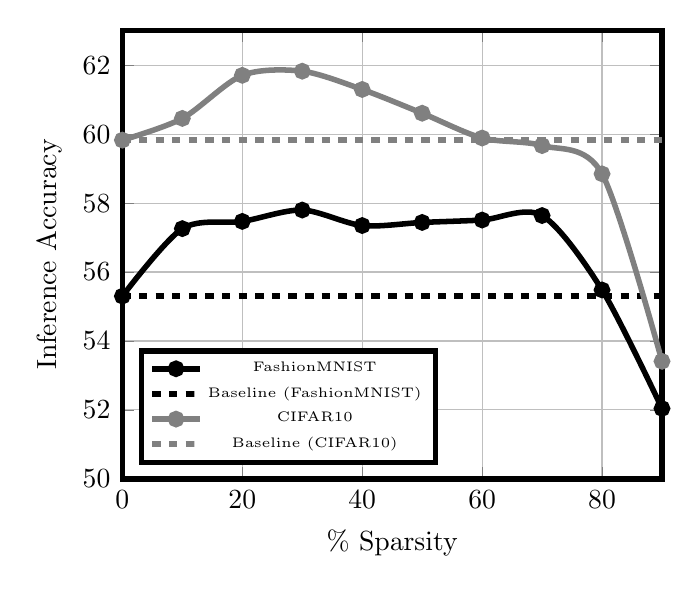
\begin{tikzpicture}
\begin{axis}[
legend style={font=\tiny},
legend pos =  south west,
line width=2.0pt,
mark size=2.0pt,
ymin=50,
xmin=0,
xmax=90,
legend entries={FashionMNIST, Baseline (FashionMNIST), CIFAR10, Baseline (CIFAR10)},
ylabel={Inference Accuracy},
xlabel={\% Sparsity},
% extra x ticks={1,10,...,400},
% extra y ticks={0,0.5,...,10},
% extra y tick labels={},
% extra x tick labels={},
% extra x tick style={grid=major},
% extra y tick style={grid=major},
grid=major
]
\addplot[
    color=black,
    solid,
    mark=*,
    mark options={solid},
    smooth
    ]
    coordinates {
    (0,55.30)(10,57.26)(20,57.47)(30,57.80)(40,57.35)(50,57.44)(60,57.51)(70,57.64)(80,55.48)(90,52.04)
      };
\addplot[
    color=black,
    dashed,
    smooth
    ]
    coordinates {
    (0,55.30)(10,55.30)(20,55.30)(30,55.30)(40,55.30)(50,55.30)(60,55.30)(70,55.30)(80,55.30)(90,55.30)
      };
\addplot[
    color=gray,
    solid,
    mark=*,
    mark options={solid},
    smooth
    ]
    coordinates {
    (0,59.83)(10,60.46)(20,61.71)(30,61.83)(40,61.30)(50,60.61)(60,59.89)(70,59.67)(80,58.85)(90,53.41)
      };
\addplot[
    color=gray,
    dashed,
    smooth
    ]
    coordinates {
    (0,59.83)(10,59.83)(20,59.83)(30,59.83)(40,59.83)(50,59.83)(60,59.83)(70,59.83)(80,59.83)(90,59.83)
      };
\end{axis}
\end{tikzpicture} &


%
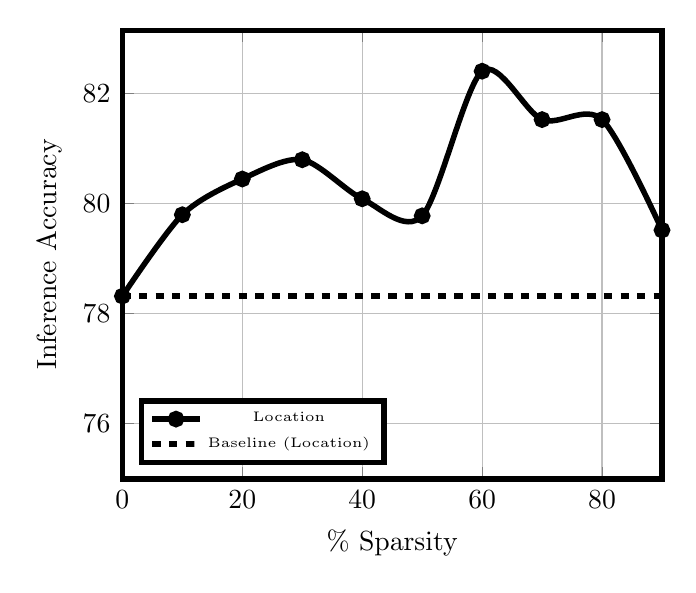
\begin{tikzpicture}
\begin{axis}[
legend style={font=\tiny},
legend pos =  south west,
line width=2.0pt,
mark size=2.0pt,
ymin=75,
xmin=0,
xmax=90,
legend entries={Location, Baseline (Location)},
ylabel={Inference Accuracy},
xlabel={\% Sparsity},
grid=major
]
\addplot[
    color=black,
    solid,
    mark=*,
    mark options={solid},
    smooth
    ]
    coordinates {
    (0,78.32)(10,79.80)(20,80.45)(30,80.80)(40,80.09)(50,79.78)(60,82.41)(70,81.53)(80,81.53)(90,79.52)
      };
\addplot[
    color=black,
    dashed,
    smooth
    ]
    coordinates {
    (0,78.32)(10,78.32)(20,78.32)(30,78.32)(40,78.32)(50,78.32)(60,78.32)(70,78.32)(80,78.32)(90,78.32)
      };

\end{axis}
\end{tikzpicture} &





%
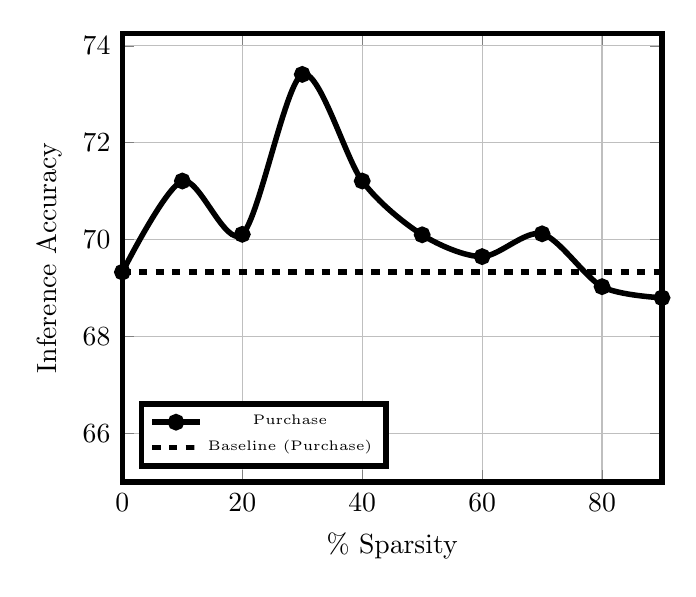
\begin{tikzpicture}
\begin{axis}[
legend style={font=\tiny},
legend pos =  south west,
line width=2.0pt,
mark size=2.0pt,
ymin=65,
xmin=0,
xmax=90,
legend entries={Purchase, Baseline (Purchase)},
ylabel={Inference Accuracy},
xlabel={\% Sparsity},
grid=major
]
\addplot[
    color=black,
    solid,
    mark=*,
    mark options={solid},
    smooth
    ]
    coordinates {
    (0,69.33)(10,71.21)(20,70.11)(30,73.41)(40,71.21)(50,70.10)(60,69.65)(70,70.12)(80,69.03)(90,68.80)
      };
\addplot[
    color=black,
    dashed,
    smooth
    ]
    coordinates {
    (0,69.33)(10,69.33)(20,69.33)(30,69.33)(40,69.33)(50,69.33)(60,69.33)(70,69.33)(80,69.33)(90,69.33)
      };

\end{axis}
\end{tikzpicture}


\end{tabular}
}
\caption{.}
\label{fig:loss}
\end{center}
\end{figure*}
